\documentclass[12pt, letterpaper, oneside]{book}

% --- Paquetes de Idioma y Formato ---
\usepackage[utf8]{inputenc}
\usepackage[T1]{fontenc}
\usepackage[spanish, es-tabla]{babel} 
\usepackage[left=3cm, right=2.5cm, top=3cm, bottom=3cm]{geometry}
\usepackage{setspace} \onehalfspacing 

% --- Matemáticas, Gráficos y Tablas ---
\usepackage{csquotes}
\usepackage{amsmath, amsfonts, amssymb}
\usepackage{graphicx}
\usepackage{float}
\usepackage{booktabs} 
\usepackage{caption}
\usepackage{booktabs}
\usepackage{longtable}
\usepackage{tabularx}
\usepackage{array}
\usepackage{caption}
\usepackage{subcaption}
\usepackage{enumitem}
\setcounter{tocdepth}{4}
\setcounter{secnumdepth}{4}



% --- Paquete para texto de relleno (Lorem Ipsum) ---
\usepackage{lipsum} 

% --- Bibliografía (IEEE) ---
\usepackage[style=ieee, backend=biber]{biblatex}
\addbibresource{references.bib}

% --- Encabezados y Pies de Página ---
\usepackage{fancyhdr}
\pagestyle{fancy}
\fancyhf{} % Borra configuraciones por defecto

% --- Configuración del ENCABEZADO (Header) ---
% Centrado, en cursivas y con el título de tu tesis
\fancyhead[C]{\textit{Auto-diseño de algoritmos en el marco de Sistemas de Auto-Ingenieria (SES)}}
\renewcommand{\headrulewidth}{0.4pt} % Línea horizontal superior

% --- Configuración del PIE DE PÁGINA (Footer) ---
\fancyfoot[L]{\thepage}           % Izquierda: Número de página (o \thepage para que sea automático)
\fancyfoot[C]{\textit{Miguel Angel Salazar Martinez}} % Centro: Nombre en cursivas
\fancyfoot[R]{\thechapter}        % Derecha: Capítulo (o Ch. \thechapter para automático)
\renewcommand{\footrulewidth}{0.4pt} % Línea horizontal inferior (como en la imagen)

% --- Ajuste de altura del encabezado ---
% A veces LaTeX da un error de "headheight is too small", esto lo corrige:
\setlength{\headheight}{15pt}

% --- Hipervínculos ---
\usepackage[colorlinks=true, allcolors=blue]{hyperref}

\begin{document}

% ---------------------------------------------------------
% SECCIONES PRELIMINARES
% ---------------------------------------------------------
\frontmatter

% --- PORTADA ---
\begin{titlepage}
    \begin{center}
        \begin{minipage}[c]{0.25\textwidth}
            \begin{center}
                
\includegraphics[width=0.80\textwidth]{figures/CINV.png} 
            \end{center}
        \end{minipage}
        \hfill
        \begin{minipage}[c]{0.74\textwidth}
            \begin{center}
                {\large \textbf{Centro de Investigación y de Estudios Avanzados\\ del Instituto Politécnico Nacional \\[0.1cm] Unidad Guadalajara}}
            \end{center}
        \end{minipage}
        
        \vspace{2cm}
        
        {\LARGE \textbf{Auto-diseño de algoritmos en el marco de Sistemas de Auto-Ingenieria (SES)}}\\[2cm]
        
        {\large Tesis que presenta:}\\[0.3cm]
        {\Large \textbf{Miguel Angel Salazar Martinez}}\\[1.2cm]
        
        {\large para obtener el grado de:}\\[0.3cm]
        {\Large \textbf{Maestro en Ciencias}}\\[1.2cm]
        
        {\large en la especialidad de:}\\[0.3cm]
        {\Large \textbf{Ingeniería Eléctrica}}\\[1.2cm]
        
        {\large Director de Tesis}\\[0.3cm]
        {\Large \textbf{Dr. Mario Angel Siller González Pico}}
    \end{center}
    \vfill 
    \noindent 
    {\large Guadalajara, Jalisco \hfill Agosto de 2026}
\end{titlepage}

\begin{titlepage}
    \begin{center}
        \vspace{2cm}
        
        {\Huge \textbf{Auto-diseño de algoritmos en el marco\\ de Sistemas de Auto-Ingenieria (SES)}}\\[2cm]
        
        {\LARGE \textbf{Tesis de Mestria en \\Ciencias Ingeniería Eléctrica}}\\[1.2cm]
        
        {\large Por:}\\[0.3cm]
        {\LARGE \textbf{Miguel Angel Salazar Martinez}}\\[0.3cm]
        {\Large Ingeniero en Sistemas Computaciones}\\
        {\Large Instituto Tecnologico de Ocotlán 2019-2023}
        \\[1.2cm]
        
        
        {\Large Becario de SECIHTI, expediente no. xxxxxxx}\\[1.2cm]
        
        {\Large Director de Tesis}\\[0.3cm]
        {\LARGE \textbf{Dr. Mario Angel Siller González Pico}}
    \end{center}
    \vfill 
    \noindent 
    {Centro de Investigación y de Estudios Avanzados del Instituto Politécnico Nacional}\\
    \noindent 
    {Unidad Guadalajara, Agosto de 2026}
\end{titlepage}

% --- RESUMEN Y AGRADECIMIENTOS ---
\chapter*{Resumen}
\addcontentsline{toc}{chapter}{Resumen}

\chapter*{Abstract}
\addcontentsline{toc}{chapter}{Abstract}

\chapter*{Dedicatoria}
\addcontentsline{toc}{chapter}{Dedicatoria}

A mi madre por ser mi ejemplo a seguir. Agradezco infinitamente tu amor y apoyo incondicional.
A mi hermana Saidy y mi hermano Diego, por impulsarme a seguir adelante y ser mi espacio seguro. A mi abuela por enseñarme lo que es ser un buen ser humano. A la vida, por permitirme llegar tan lejos. 

\chapter*{Agradecimientos}
\addcontentsline{toc}{chapter}{Agradecimientos}

\noindent A todos los que me apoyaron en el camino y me ayudaron en esta travesía del posgrado.\\
A mi asesor de tesis, el Dr. Mario Siller, por todo el apoyo durante el desarrollo del plan de estudios.\\
A mi querida familia, a mi madre, a mi padre, a mis hermanos, a mis abuelos, a mis tios y primos que tanto me han apoyado.\\
Al grupo de redes de CINVESTAV Guadalajara, que más que grupo, es una familia.\\
A los doctores del área de computación, por compartir su conocimiento, consejos y, sobre todo, por cultivar la tenacidad. Esa que no aparece en la rubrica, pero que resulta indispensable para llegar hasta aquí.\\
A todos mis amigos (incluyendo los compis y roomies) especialmente a los miembros del laboratorio de computación, por esas largas charlas, orientación, momentos de calidez y de recreación.\\
A todos mis maestros, quienes me educaron en toda mi vida académica y nunca desistieron al enseñarme.\\
Entre ellos destaco a la profesora Aurora Berenice Navarro Nuñez, por darme el apoyo que necesite al momento de ingresar a este posgrado.\\
A todos aquellos que creyeron en mí.\\
Finalmente, quiero agradecer a la SECIHTI por el apoyo económico brindado, con el cual se logró concluir esta maestría.\\
Muchas Gracias a todos.
\vfill 
    \noindent 
    {Quiero aclarar que no nombré a todos los involucrados, no por falta de gratitud, sino porque en extensión, los agradecimientos serian inmensos.}\\

% --- ÍNDICES ---
\tableofcontents
\listoffigures
\listoftables

% ---------------------------------------------------------
% CUERPO DE LA TESIS
% ---------------------------------------------------------
\mainmatter

% Si prefieres usar archivos separados, comenta las líneas de abajo y usa:
% \include{capitulos/01_introduccion}
% Por ahora, incluyo los capítulos aquí mismo para que sea una plantilla rápida.

\chapter{Introducción}
El desarrollo de sistemas de software contemporáneos está intrínsecamente ligado a la evolución de la Ingeniería de Software. A lo largo de las últimas décadas, se ha evidenciado que las actividades de mantenimiento, actualización y evolución de artefactos de software representan una etapa con alto coste en términos de capital humano, tiempo de desarrollo y recursos financieros \cite{PerezCarrillo2026}. Para mitigar esta dependencia, el paradigma de los Sistemas de Auto-Ingeniería (\textit{Self-Engineering Systems} - SES) introduce un marco conceptual y una meta-arquitectura que habilitan a los sistemas de software para ejecutar modificaciones autónomas sobre sí mismos, abriendo la posibilidad de realizar procesos de auto-evolución o metamorfosis \cite{perez2024}. El propósito fundamental de un sistema SES es gestionar y ejecutar su propio proceso de ingeniería más allá de su ciclo de vida convencional, prescindiendo de la intervención humana.

Dentro de este ciclo autónomo, una de las actividades fundamentales y de mayor impacto metodológico es la ingeniería de diseño. Esta fase es crítica debido a que es la encargada de traducir los requerimientos abstractos del entorno en especificaciones técnicas detalladas, estructuras de datos, interfaces y asignación de componentes indispensables para la posterior implementación y ejecución del sistema. En el contexto de los sistemas SES, automatizar esta etapa ---es decir, dotar al sistema de capacidades de auto-diseño--- implica que la plataforma no solo reaccione a fallos, sino que sea capaz de reconfigurar conceptualmente su propia lógica operacional de manera válida, segura y coherente con las decisiones arquitectónicas previas.

Sin embargo, replicar la totalidad del ciclo de ingeniería de diseño constituye un desafío multidimensional. Por ello, y considerando las delimitaciones temporales propias de una investigación de posgrado, este trabajo se acota estrictamente a trabajar con cajas negras y unicamente explicar la actividad del \textit{auto-diseño de algoritmos}. Bajo este alcance, la resolución de dicha actividad se aborda mediante un enfoque formal de asociación problema-solución. Este mecanismo se operativiza a través de una especificación ontológica que proporciona una taxonomía estructurada de problemas, permitiendo al sistema clasificar un requerimiento dinámico y determinar la solución algorítmica idónea para su posterior implementación autónoma.

\section{Planteamiento del Problema}
El diseño de software es una etapa crucial en el ciclo de desarrollo que abarca desde las abstracciones de alto nivel ---representadas formalmente en las distintas vistas de la arquitectura de software \cite{Kruchten1995The}--- hasta la especificación granular de sus componentes. Tradicionalmente, esta actividad demanda un consumo elevado de recursos organizacionales y un esfuerzo cognitivo humano significativo. Aunque las metodologías han evolucionado hacia el paradigma de la Ingeniería de Software 3.0 ---donde los sistemas basados en agentes autónomos han ganado terreno \cite{li2025riseaiteammatessoftware}---, los sistemas actuales carecen de mecanismos para modificar de forma autónoma su lógica algorítmica interna sin alterar o comprometer las estructuras arquitectónicas preexistentes.

El problema técnico radica en la ausencia de un mecanismo capaz de acoplar un agente diseñador de algoritmos con las actividades de diseño previas (arquitectura, componentes y estructuras de datos). Al no existir un modelo de abstracción que trate a estas capas previas como una entidad de tipo caja negra, los sistemas adaptativos no pueden actualizar su lógica operacional de manera aislada y segura ante cambios dinámicos en sus requerimientos. Para resolver esta limitación, se requiere un modelo donde la ontología actúe como el puente semántico entre el espacio del problema (los nuevos requerimientos clasificados taxonómicamente) y el espacio de la solución (los algoritmos disponibles), permitiendo que la selección e integración ocurran de forma autónoma y sin romper las interfaces preexistentes.

\section{Motivación}
La motivación central de esta investigación radica en la necesidad de desarrollar sistemas de software con un alto grado de autonomía, capaces de autodiseñar su propia lógica interna cuando las demandas del entorno lo requieran. Al automatizar la generacion de artefactos de diseño y la selección de algoritmos mediante el uso de ontologías y agentes de diseño, se establece un habilitador crítico para la evolución y metamorfosis de los sistemas SES \cite{perez2024}. Este enfoque no solo reduce la dependencia del factor humano en entornos críticos y dinámicos, sino que optimiza los costos operativos asociados al mantenimiento evolutivo del software, transformando la adaptación heurística en un proceso de inferencia lógica y clasificación formal.
\section{Objetivos}

\subsection{Objetivo General}

Desarrollar un marco conceptual para el diseño automatizado en sistemas de auto-ingenieria, el cual sea capaz de actualizar o implementar desiciones de diseño ante cambios en los requerimientos, abstrayendo las actividades de diseño previas (arquitectura, interfaces y estructuras de datos) mediante un modelo de interacción de caja negra con un agente diseñador de caja blanca.


\subsection{Objetivos Específicos}
\begin{itemize}
    
\item Sintetizar el estado del arte en materia de diseño de software automatizado y selección algorítmica autónoma, mediante la ejecución y análisis de una Revisión Sistemática de la Literatura (RSL), con el fin de identificar las tendencias, limitaciones y brechas de conocimiento existentes.

\item Formalizar y conceptualizar el término ``autodiseño`` (Self-Design) en el contexto de los sistemas de software, clasificando sus tipologías y variantes taxonómicas a partir de las capacidades y la información disponible en el entorno del sistema.

\item Caracterizar los mecanismos de actualización e implementación autónoma de algoritmos, analizando los criterios técnicos y las restricciones operacionales requeridas para su ejecución sin intervención humana.

\item Diseñar una meta-arquitectura que gobierne la gestión, sustitución e integración de cambios algorítmicos, definiendo explícitamente las interfaces de comunicación tipo caja negra entre las estructuras de diseño preexistentes y el agente diseñador propuesto.

\item Validar la viabilidad y efectividad del marco de trabajo desarrollado a través del despliegue de casos de estudio en escenarios experimentales controlados, evaluando su capacidad de adaptación frente a la variabilidad de requerimientos.

\end{itemize}



\section{Hipótesis}

Es posible dotar a un sistema de un mecanismo que le permita analizar cambios en sus requerimientos y gestionar de manera autónoma el rediseño de sí mismo, ya sea mediante la generación de un nuevo diseño o la adaptación del diseño existente cuando este continúe satisfaciendo los nuevos requerimientos.


\section{Estructura del documento de la Tesis}


La estructura de este documento se organiza en seis capítulos interconectados que guían el desarrollo de la investigación. 

El \textbf{Capítulo 1} establece la base del estudio mediante la introducción del problema, la motivación, los objetivos, las hipótesis y el contexto general. El \textbf{Capítulo 2} expone los fundamentos teóricos indispensables para la comprensión del trabajo, abordando conceptualizaciones clave sobre Sistemas de Auto-Ingeniería (SES, por sus siglas en inglés), automatización, diseño de software y selección algorítmica. Posteriormente, el \textbf{Capítulo 3} ofrece una revisión y análisis crítico del estado del arte, identificando las tendencias actuales, los enfoques metodológicos existentes, así como sus limitaciones y brechas de conocimiento. En el \textbf{Capítulo 4 }se detalla la propuesta central de esta investigación, especificando su metodología, conceptualización, arquitectura y los mecanismos de selección automática diseñados. La validación experimental de dicha propuesta se describe en el \textbf{Capítulo 5} a través de casos de estudio, la simulación de escenarios y el análisis riguroso de los resultados obtenidos. Finalmente, el \textbf{Capítulo 6} cierra el documento exponiendo las conclusiones generales, las contribuciones principales de la investigación, sus limitaciones intrínsecas y las directrices sugeridas para el trabajo futuro.

%%%%%%%%%%%%%%%%%%%%%%%%%%%%%%%%%%%%%%%%%%%%%%%%%%%%%%%%%%%%

\chapter{Marco Teórico}

Este capitulo engloba toda la teoria que sustenta la investigacion y pos ende la propuesta.

\section{Sistemas de Auto-Ingenieria}
%\cite perez
En \cite{perez2024} se aborda el hecho de que los mismo sistemas no terminen en desecho si no, que sin intervención humana continuen su operacion evolucionando o en su defecto sufran una metamorfosis dando pie a un nuevo sistema, esta perspectiva se conoce como el marco de los sistemas de auto-ingenieria.
Los SES contemplan un proceso muy similar a la ingenieria de software tradicional, es decir las actividades como lo son ingenieria de requerimientos, diseño, implementacion, pruebas, etc.\cite{sommerville2011software} tambien estan contempladas. Para este trabajo unicamente nos enfocamos a la ingenieria de diseño.

\subsection{Marco de Sistemas de Auto-Ingeniería}

Los SES cuentan con el ether, el centro de operacion de estos sistemas, recordando el hecho de la existencia de dos momentos clave, la evolucion y la metamorfosis, Un sistema SES busca gestionar y ejecutar su propio proceso de ingenieria mas alla de su ciclo de vida convencional, prescindiendo de la intervencion humana.


\section{Actividades de diseño}
%\cite sommerville
Las actividades principales de la ingenieria de diseño son:
Diseño de Arquitectura
Diseño de Interfaces
Diseño de componentes
Diseño de Estructuras de datos
Diseño de Algoritmos


\subsection{Diseño de Arquitectura}



\subsection{Diseño de Interfaces}



\subsection{Diseño de Componentes}



\subsection{Diseño de Estructuras de datos}



\subsection{Diseño de Algoritmos}



\section{Diseño Automatizado de Algoritmos}



\section{Ontología para selección automática de algoritmos}



\chapter{Estado del Arte}

Este capitulo presenta y analiza lo que existe en la literatura cientifica acerca del diseño automatizado o auto-diseño.
Incluyen definiciones, tecnicas y marcos de trabajo, 




\section{Conceptualizacion del Auto-diseño}

\shorthandoff{"}
Sin lugar a dudas el trabajo de \cite{Porter2024SelfDesigning} es el trabajo mas cercano al auto-diseño, concibe al Self-Designing Software como al propio software convertido en un miembro activo de su equipo de diseño. La tecnica principal es el "Hot-Swapping", este intercambio en caliente permite intercambiar componentes de software en un sistema vivo de forma segura, con el uso de "building blocks", estos bloques de construccion estan validados y cuentan con interfaces especificas para su acople o desecho.
 
 Sin embargo no cubre el diseño como un conjunto de actividades que nos entregan artefactos de diseño \cite{sommerville2011software} es asi que en una busqueda mas a profundidad mediante una revision sistematica de literatura, encontramos actividades total o parcialmente automatizadas que buscan satisfacer el diseño automatizado.
 
 El trabajo de \cite{StratosIdreos2019LearningData} describe una metodología para automatizar el diseño de estructuras de datos a través de la síntesis de estructuras personalizadas. En lugar de depender de diseños tradicionales fijos, este enfoque construye estructuras a la medida partiendo de un conjunto de primitivas de diseño fundamentales lógicas y físicas clasificadas en su "Tabla Periódica de las Estructuras de Datos" \cite{idreos2018periodic}. El conjunto combinatorio de estas primitivas conforma un vasto "espacio de diseño" en el cual se evalúan rigurosamente las restricciones de rendimiento y utilización de recursos. Tras este análisis, el diseño óptimo es enviado a un generador de código para sintetizar el diseño en código fuente ejecutable para el sistema final.
 %Loncaric,Zhao, Wenjie,zhnag, aurora R, Weyns, Affonso, GIl, Ageloupulos
 De igual manera (en la etapa de diseño de estructuras de datos) la herramienta COZY\cite{loncaric2016Datastructure} y mejorada en \cite{loncaric2018Generalizeddata}, presentan una solucion muy parecida a la mencionada previamente, la entrada de esta herramienta consta de el conjunto de instrucciones que describan que tipo de datos logicos (usuario, grupos, membresias), que se busca en esos datos y que operaciones implican (actualizar, borrar, etc), para asi llegar a la estructura optima. Esto se lleva a cabo a traves de un proceso iterativo, puede llegar a crear estructuras intermedias que no son las mejores, asi que   se evalua la eficiencia y eficacia de las mismas, tiene un mecanismo de verificacion y garantias, mediante inferencia busca contraejemplos (apoyado por el resolvedor SMT Z3) y por ultimo un implementador de codigo.
\shorthandon{"}
\section{Automatización del Diseño}



\subsection{Autodiseño basado en Inteligencia Artificial}



\subsection{Autodiseño bio-inspirado}



\subsection{Autodiseño basado en modelado de agentes}



\subsection{Autodiseño basado en el reuso y busqueda}



\section{Conceptos emergentes similares al auto-diseño}


\section{Comparacion de trabajos}



\chapter{Propuesta}

\section{Metodologia}
La metodologia consta de dos  etapas principales, la primera que fue realizar una revision sistematica de literatura sobre tecnicas, marcos de trabajo y demas propuestas que llevaran a cabo el autodiseño, esta misma se llevo a cabo siguiendo la metodologi prisma, los resultados obtenido ayudaron a fundamentar la toma de decision para construir la propuesta.
La siguiente etapa fue la construccion de un sistema multiagentes, se compararon diferentes metodologias, pero se decanto por prometheus ya que implementa los conceptos BDI de manera natural, la comparacion con metodologias esta dada con (Gaia, Tropos, Mase, O-mase, Adelfe, Pass)


\subsection{Revision Sistematica de literatura}

El primer paso para desarrollar y fundamentar mi propuesta fue realizar un revision sistematica de literatura, en la que siguiendo los lineamientos PRISMA \cite{Pagen2020PRISMA}, con este proceso estructurado se realizo la revision de manera exhaustiva, el objetivo principal de esta Systematic Literature Review (SLR), es conocer como se ha automatizado el diseño de sistemas, conocer el estado del arte permite reconocer vacios en el mismo.
\subsubsection{Formulación preguntas de investigación}

La formulacion de una pregunta o preguntas de investigación en cualquier investigación es la piedra angular de la misma, en una SLR no es la excepción, para esto se utilizo el marco de trabajo PICO \cite{barbaraGuidelines}, La Poblacion (P), habarca los procesos de diseño de software, desde las tareas tradicionales automatizadas, hasta el auto-diseño bajo el marco de los sistemas de autoingenieria (SES) o que tengan relacion directa con ellos. La intervencion (I) se refiere a todos los enfoques automatizados, autonomos o impulsados por IA dentro de la basta literatura, para apoyar a dichas actividades. Estos enfoques comprenden modelos, tecnicas y mecanismos destinados a permitir que los sistemas generen, evaluen, o evoluciones artefactos de diseño de manera autonoma. La Comparacion (C), implica un analisis comparartivo entre las metodologias o tecnicas convencionales, contra enfoque progresivamente automatizados. Finalmente, el resultado previsto, denominado Resultado (Outcome en ingles), destaca en una sintesis sistematica del conocimiento existente para mapear estae volucion tecnologiaca, evaluar las teorias e identificar las brechas de investigacion pendientes que obstaculizan la realizacion de un verdadero auto-diseño.

Con base a esta formulacion las siguientes preguntas son propuestas:

\begin{itemize}
	\item \textbf{RQ1:} ¿De que maneras se han automatizado o hecho autónomos los procesos tradicionales de ingenieria de diseño de software?
	\item \textbf{RQ2:} ¿Que terminos o conceptos emergentes son equivalentes o cercanos a una actividad de diseño totalmente autonoma?
	\item \textbf{RQ3:} ¿Como se ha abordado el  \textbf{autodiseño} de sistemas en el contexto de los SES?
\end{itemize}

\subsubsection{Estrategia de busqueda}
Para contestar a la primer pregunta de investigacion (RQ1), el analisis fue estructurado alrededor de las actividades en el diseño de software, considerando su correspondencia con enfoques automaticos o autonomico, las etapas se muestran en la tabla ~\ref{tab:etapas_diseno}.

\begin{table}[H]
	\centering
	\caption{Actividades de diseño y sus correspondientes artefactos de diseño.}
	\label{tab:etapas_diseno}
	\begin{tabular}{@{}ll@{}}
		\toprule
		\textbf{Actividades de diseño} & \textbf{Artefactos de diseño} \\ \midrule
		Diseño de Arquitectura & Arquitectura del sistema\\
		Diseño de interfaz & Especificacion de interfaces \\
		Diseño de componentes & Especificacion de componentes\\
		Diseño de estructuras de datos & Especificacion de estructuras de datos \\
		Diseño de algoritmos & Especificacion de algoritmos \\
		\bottomrule
	\end{tabular}
\end{table}

Esta descomposicion facilita eavaluar en que medida cada fase del diseño ha sido reinterpretada, respaldada o automatizada bajo los principios de automatizacion de autogestion. Esto ofrece una vision amplia del diseño en nuestra busqueda. De tal manera que una busqueda granular se consigue con sub-preguntas de investigacion, al final se contesta la RQ1.

\begin{itemize}
	
	\item \textbf{SRQ1.1} ¿De qué manera se ha conceptualizado, implementado o evaluado el autodiseño arquitectónico o la automatización del diseño arquitectónico en la literatura?
	
	\item \textbf{SRQ1.2} ¿Cómo se ha generado o abordado la noción de autodiseño de interfaces o de diseño automatizado de interfaces en la investigación existente?
	
	\item \textbf{SRQ1.3} ¿En qué medida se ha explorado y tratado el autodiseño de componentes o el diseño automatizado de componentes en estudios previos?
	
	\item \textbf{SRQ1.4} ¿Cómo se han definido e investigado en la literatura los enfoques sobre el autodiseño de estructuras de datos o el diseño automatizado de estructuras de datos?
	
	\item \textbf{SRQ1.5} ¿Cómo se ha abordado el autodiseño de algoritmos o el diseño automatizado de algoritmos?
	
\end{itemize}

Para proveer de una respuesta mas comprensiva a la segunda pregunta de investigacion (RQ2), se realizo una busqueda exploratoria de manera exploratoria, usando terminologia reciente y emergente. Este paso apunta a identificar conceptos e investigaciones que de una manera no explicita busca el auto-diseño. como resultado tenemos topicos como diseño evolucionario de systemas de software, diseño generativo en software, automatizacion del diseño de software e inteligencia artificial para ingenieria de software (AI4SE), estos topicos se añadieron a la estrategia de busqueda.
Por ultimo, la manera de abordar la tercer pregunta de investigacion (RQ3), se adopto una estrategia dirigida por el concepto clave de auto-diseño, algo que de manera explicita nos dirigiera a esto. asi que se suman los siguiente terminos:
Auto-diseño,  Systemas de Auto-Arquitectura y Sistemas autosuficientes.

Las busquedas de la SLR fue realizada en cuatro bases de datos de alto impacto en el campo de la ingenieria de software: Scopus, Web of Science, IEEE Xplore y ACM Digital Library. 
Estas plataformas se seleccionaron debido a la disponibilidad de acceso institucional completo y a su amplia cobertura de publicaciones revisadas por pares, incluidos artículos de revistas, actas de conferencias y capítulos de libros relevantes para la inteligencia artificial, la ingeniería de software y los sistemas autónomos y autonómicos.
 Google Scholar si bien es un buen motor de busqueda, no es una base de datos de manera directa y presenta limitaciones en la replicabilidad de las busquedas, por lo tanto no fue una fuente primaria de busqueda \cite{Gusenbauer2020}, sin embargo en el proceso de bola de nieve (snowballing) si se uso para la busqueda de las citas, tanto de entrada como de salida.
 
 Las estrategias de búsqueda se elaboraron sistemáticamente combinando términos relacionados con el tema mediante operadores booleanos (\texttt{AND}, \texttt{OR}) para estructurar explícitamente sus relaciones lógicas. La búsqueda se restringió al campo \texttt{TITLE-ABS-KEY} con el fin de aumentar la precisión conceptual y reducir el ruido en la recuperación de información. Posteriormente, se aplicaron criterios de inclusión y exclusión predefinidos para refinar y validar el conjunto de estudios resultante. Un ejemplo de una consulta completa esta escrita en la tabla~\ref{tab:example_query}.
 
 \shorthandoff{"}
 \begin{table}[ht]
 	\centering
 	\caption{Example of Complete Search Query (Scopus)}
 	\label{tab:example_query}
 	\begin{tabularx}{\textwidth}{|l|X|}
 		\hline
 		\textbf{Database} & Scopus \\ \hline
 		\textbf{Search Field} & TITLE-ABS-KEY \\ \hline
 		\textbf{Time Range} & 2015--2026 \\ \hline
 		\textbf{Subject Areas} & Computer Science (COMP), Engineering (ENGI) \\ \hline
 		\textbf{Complete Query} &
 		\texttt{TITLE-ABS-KEY ((("self-architecting"\ OR "self architectural"\ OR\ "\ auto-architecting"\ OR\ "auto architectural")\ W/3\ "system*")\ OR\ (("self-architectural"\ OR\ "auto-architectural")\ W/3 "design"))\ AND\ PUBYEAR\ >\ 2014\ AND\ PUBYEAR\ <\ 2027\ AND\ (LIMIT-TO\ (SUBJAREA,\ "COMP")\ OR\ LIMIT-TO (SUBJAREA,\ "ENGI"))} \\ \hline
 	\end{tabularx}
 \end{table}
 
 Las consultas presentadas a continuacion corresponden a un conjunto resumido de expresiones que inicialmente fueron ejecutadas en Scopues, y posteriormente adaptadas a las sintaxis especificas de las diferentes bases de datos, se listan las consultas en la tabla~\ref{tab:queries}.
 
 
 
  \begin{table}[H]
 	\centering
 	\caption{Resumen de las consultas en Scopues (Obviando los filtros temporales y de dominio para mantener la brevedad).}
 	\label{tab:queries}
 	\begin{tabular}{|@{} p{0.2\textwidth} | p{0.75\textwidth} @{}|}
 		\toprule
 		\textbf{Topic/filter name} & \textbf{Summarized Query (Field: TITLE-ABS-KEY)} \\ \midrule
 		1. Self-Architecting Systems & ("self-architecting system*" OR "auto-architecting system*" OR "self-architectural design" OR "auto-architectural design") \\ \hline
 		2. Self-Design & ("self-design" OR "self design" OR "auto-design" OR "auto design" OR "self software design" OR "auto software design") \\ \hline
 		3. Evolutionary Design in Software Systems & (("evolutionary design" OR "evolutionary software design") AND ("software system*" OR "software engineering")) \\ \hline
 		4. Generative Design SW Systems & (("generative design" OR "generative software design") AND ("software system*" OR "software engineering")) \\ \hline
 		5. Software Design Automation & ("software design automation" OR "design automation in software engineering" OR "automated software design" OR "AI for software design") \\ \hline
 		6. Self-Sufficient Systems & ("self-sufficient system*" OR "autonomous self-sufficient software" OR "self-sufficient software system*") \\ \hline
 		7. AI for Software Engineering & (("AI for software engineering" OR "artificial intelligence in software engineering" OR "machine learning in software engineering")) \\ \hline
 		8. Self/Auto-Architectural Design & ("self-architectural design" OR "auto-architectural design" OR "self adaptive architecture" OR "self-adaptive design") \\ \hline
 		9. Self/Auto-Interface Design & ("self-interface design" OR "auto-interface design" OR "autonomous interface design" OR "adaptive interface design") \\ \hline
 		10. Self/Auto-Component Design & ("self-component design" OR "auto-component design" OR "autonomous component design" OR "self-generated component*") \\ \hline
 		11. Self/Auto-Data S. Design & ("self-data structure design" OR "auto-data structure design" OR "autonomous data structure" OR "self-optimizing data structure*") \\ \hline
 		12. Self/Auto-Algorithm Design & ("self-algorithm design" OR "auto-algorithm design" OR "autonomous algorithm" OR "automated algorithm" OR "generative algorithm design" OR "AI-based algorithm") \\ \bottomrule
 	\end{tabular}
 \end{table}
 \shorthandon{"}
 
Las consultas fueron ejecutadas de manera independiente y posteriormente los resultados fueron unificados (eliminando duplicados). El conjunto final de artículos formaron los \textit{estudios iniciales seleccionados} de esta revision, recordando que fueron filtrados mediante los criterios de invlusion y exclusion descritos a continuacion.

\subsubsection{Criterios de Inclusion y de exclusion}

Para garantizar la calidad y relevancia de los estudios seleccionados, se establecen criterios explicitos de inclusion y exclusion de acuerdo al objetivo de esta revision, la cual se centra en la automatizacion del diseño en el marco de los SES.

Criterios de inclusion

\begin{itemize}
	\item \textbf{CI1: Periodo Temporal.} publicaciones desde  \textbf{2015 hasta Marzo de 2026}. Un rango inicial (2005 -- 2025) fue considerado, pero se actualizo para buscar tecnicas y avances en el area de la Inteligencia Artificial, evadiendo la literatura del \textit{computo autonomico} para enfocarnos unicamente en los sistemas de autoingenieria.
	\item \textbf{CI2: Idioma.} Solo artuculos en \textbf{Ingles} fueron incluidos para alinearnos con el lenguajes mas adoptado en la divulgacion cientifica en el mundo.
	\item \textbf{CI3: Disponibilidad y Claridad.} los estudios deben proveer \textbf{acceso completo} y una \textbf{metodologia claramente definida} para permitir un analisis comprensivo y total de los mismo.
	\item \textbf{CI4: Dominio especifico.} Unicamente investigaciones en el campo de la \textbf{Ingenieria de software} que aborde de manera explicita o de manera indirecta cubra lo que es el auto-diseño de una manera unificada como proceso total o parcial.
	\item \textbf{CI5: Relevancia Científica.} Seleccion  de estudios que han demostrado impacto en la comunidad cientifica a traves de las citas, mientras se busca balancear este criterio, evaluando publicaciones reciente que no tienen un acumulado de citas pero si un gran contribucion teorica o tecnica en el tema.
\end{itemize}


Criterios de exclusion

Los siguientes criterios fueron usados para filtrar articulos que no coincidian con los requerimientos de la investigacion:

\begin{itemize}
	\item \textbf{CE1: Duplicasion.} \textbf{publicaciones duplicadas} o \textbf{multiples versiones} del mismo estudio; en cuyos casos, solo el mas completo o version mas reciente sera considerada.
	\item \textbf{CE2: Tipo de Documento.} \textbf{Documentos incompletos}, \textbf{resumenes extendidos}, o \textbf{publicaciones de posters} que carecen de suficiente detalle técnico para su evaluación.
	\item \textbf{EC3: Irrelevancia Disciplinaria.} estudios fuera del dominio de \textbf{Ingenieria de Software} sin un enlace directo al auto-diseño.
	\item \textbf{CE4: Deficiencias Metodologicas.} estudios que carezcan de \textbf{rigor metodologico}, particularmente lo que no tienen una clara descripcion de las tecnicas propuestas, algoritmos o ceonceptos.
\end{itemize}


Estos filtros (revisar Tabla~\ref{tab:criterios}) permiten la identificacion de estudios representativos y de alta calidad, centrados en avances recientes en el ambito conceptual y practicos en el area de auto-diseño y auto-ingenieria, garantizando así la validez y relevancia de esta revisión sistemática de la literatura (este capitulo en particular).

\vspace{0.5cm}

\begin{table}[H]
	\centering
	\caption{Resumen de los criterios de inclusion y exclusion}
	\label{tab:criterios}
	\begin{tabular}{p{0.25\textwidth} p{0.65\textwidth}}
		\toprule
		\textbf{Tipo} & \textbf{Criterio} \\
		\midrule
		\textbf{Inclusion} & \textbf{CI1:} Publicaciones entre 2015 y 2025. \\
		& \textbf{CI2:} Publicaciones en Ingles. \\
		& \textbf{CI3:} Disponibilidad completa con metodologia detallada.\\
		& \textbf{CI4:} Centrado unicamete en software engineering, self-engineering, or self-design. \\
		& \textbf{CI5:} Estudios relevantes con contribuciones recientes o numero de citas destacables. \\[0.2cm]
		\textbf{Exclusion} & \textbf{CE1:} Publicaciones duplicadas o multiples versiones del mismo estudio. \\
		& \textbf{CE2:} Resumenes, posters o documentos incompletos.\\
		& \textbf{CE3:} Estudios fuera del dominio de los sistemas de software.\\
		& \textbf{CE4:} Trabajos con falta de detalles en su metodologia o rigor cientifico.\\
		\bottomrule
	\end{tabular}
\end{table}

\subsubsection{Proceso de seleccion de estudios}

Este bloque describe como fue la seleccion de estudios siguiendo las pautas de PRISMA.
La Figura~\ref{fig:SearchProcess} ilustra el flujo general de identificación de estudios, cribado (aplicación de criterios de inclusión y exclusión), evaluación de elegibilidad (lectura del resumen y, posteriormente, del documento completo) e inclusión final. Los artículos semilla (conjunto inicial) se seleccionaron a partir de los estudios que cumplían los criterios de inclusión y obtuvieron las puntuaciones más altas en la evaluación de calidad durante la búsqueda inicial en bases de datos. Posteriormente, se identificaron estudios adicionales mediante la técnica de bola de nieve (hacia atrás y hacia adelante), siguiendo las directrices propuestas por \cite{Wohlin2014}. Este proceso iterativo consistió en examinar las listas de referencias de los artículos semilla (bola de nieve hacia atrás) e identificar los artículos que los citaban (bola de nieve hacia adelante), aplicando los mismos criterios de inclusión y exclusión en cada iteración.

\begin{figure}[H]
	\centering
	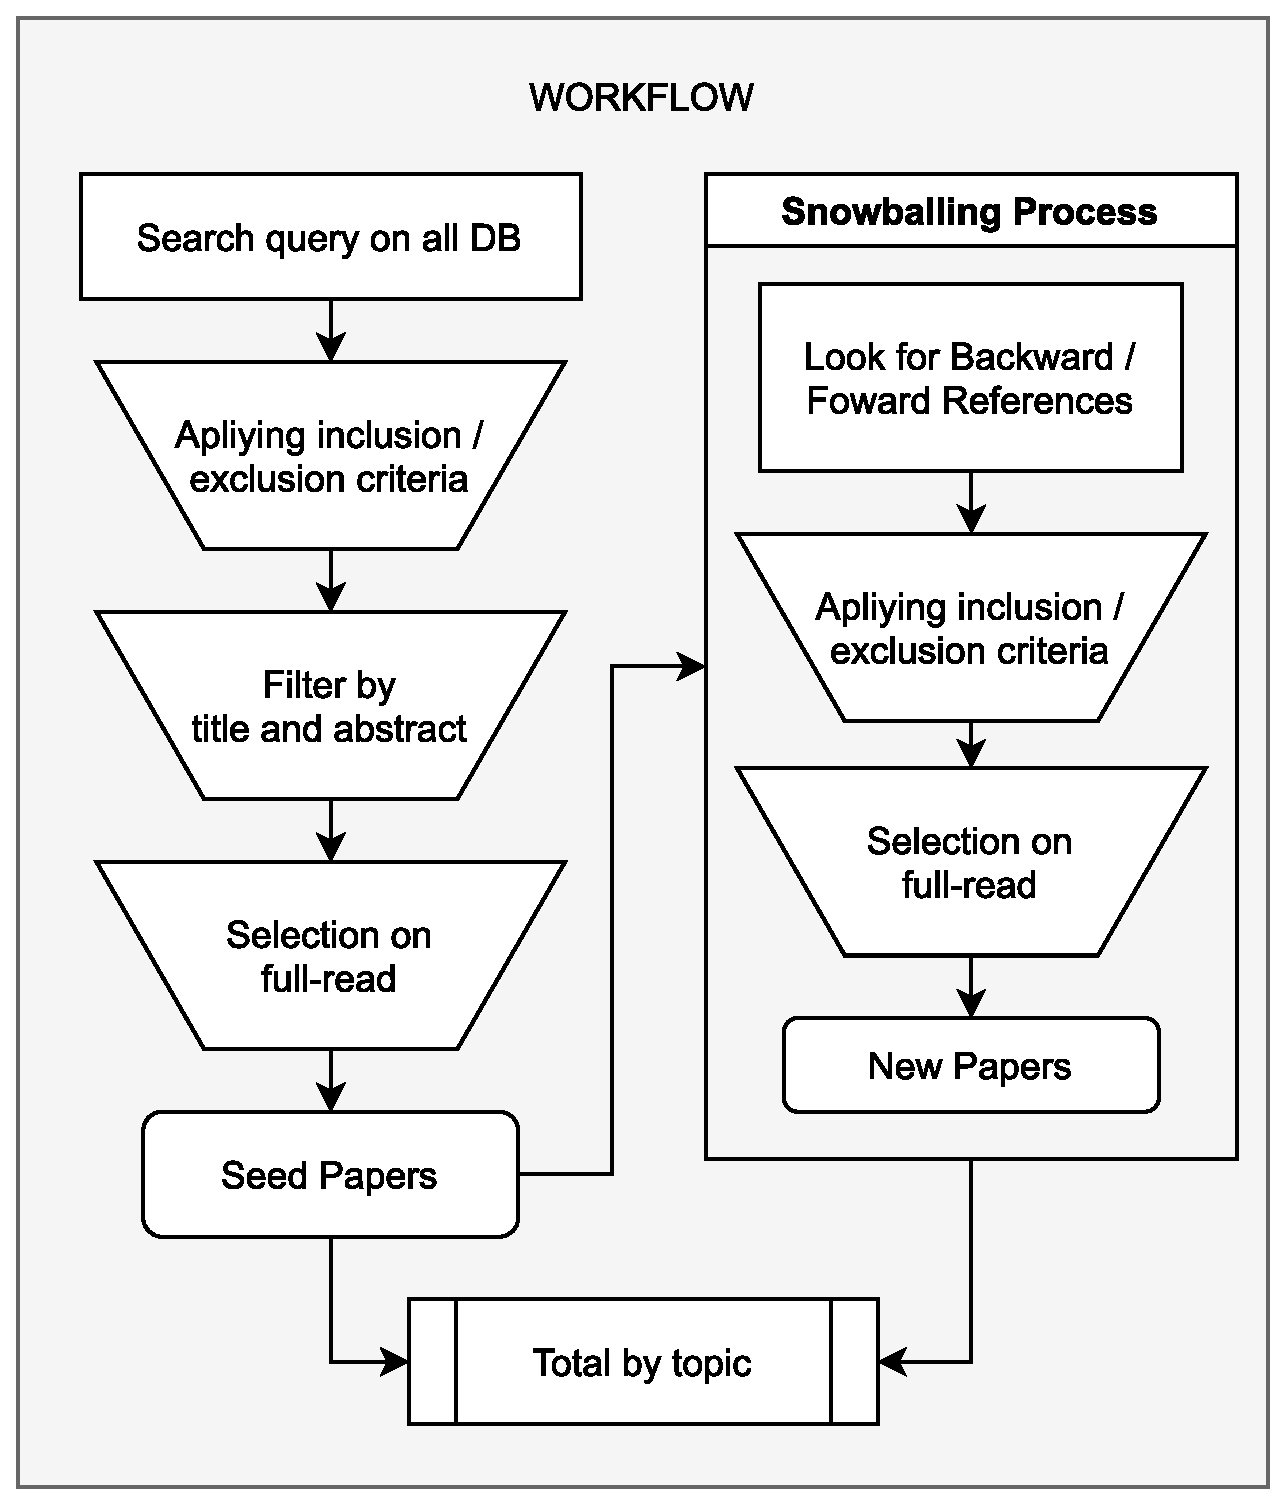
\includegraphics[width=0.7\textwidth]{figures/Fig1_Workflow.eps}
	\caption{Review process flow chart based on PRISMA.}
	\label{fig:SearchProcess}
\end{figure}

Para complementar el flujo de PRISMA, se añade una vista preelimiar a manera de cuantificar los resultados, así detallar los los estudios seleccionados por cada etapa del proceso y especificando el topico en particular. Esta representación permite comprender mejor cómo el conjunto inicial de estudios recuperados se refinó progresivamente hasta llegar a los estudios seleccionados finalmente y analizados en esta revisión. La Figura~\ref{fig:Cribado} resume este proceso mediante la especificacion explicita del umero de articulos por cada etapa de seleccion.

\begin{figure}[H]
	\centering
	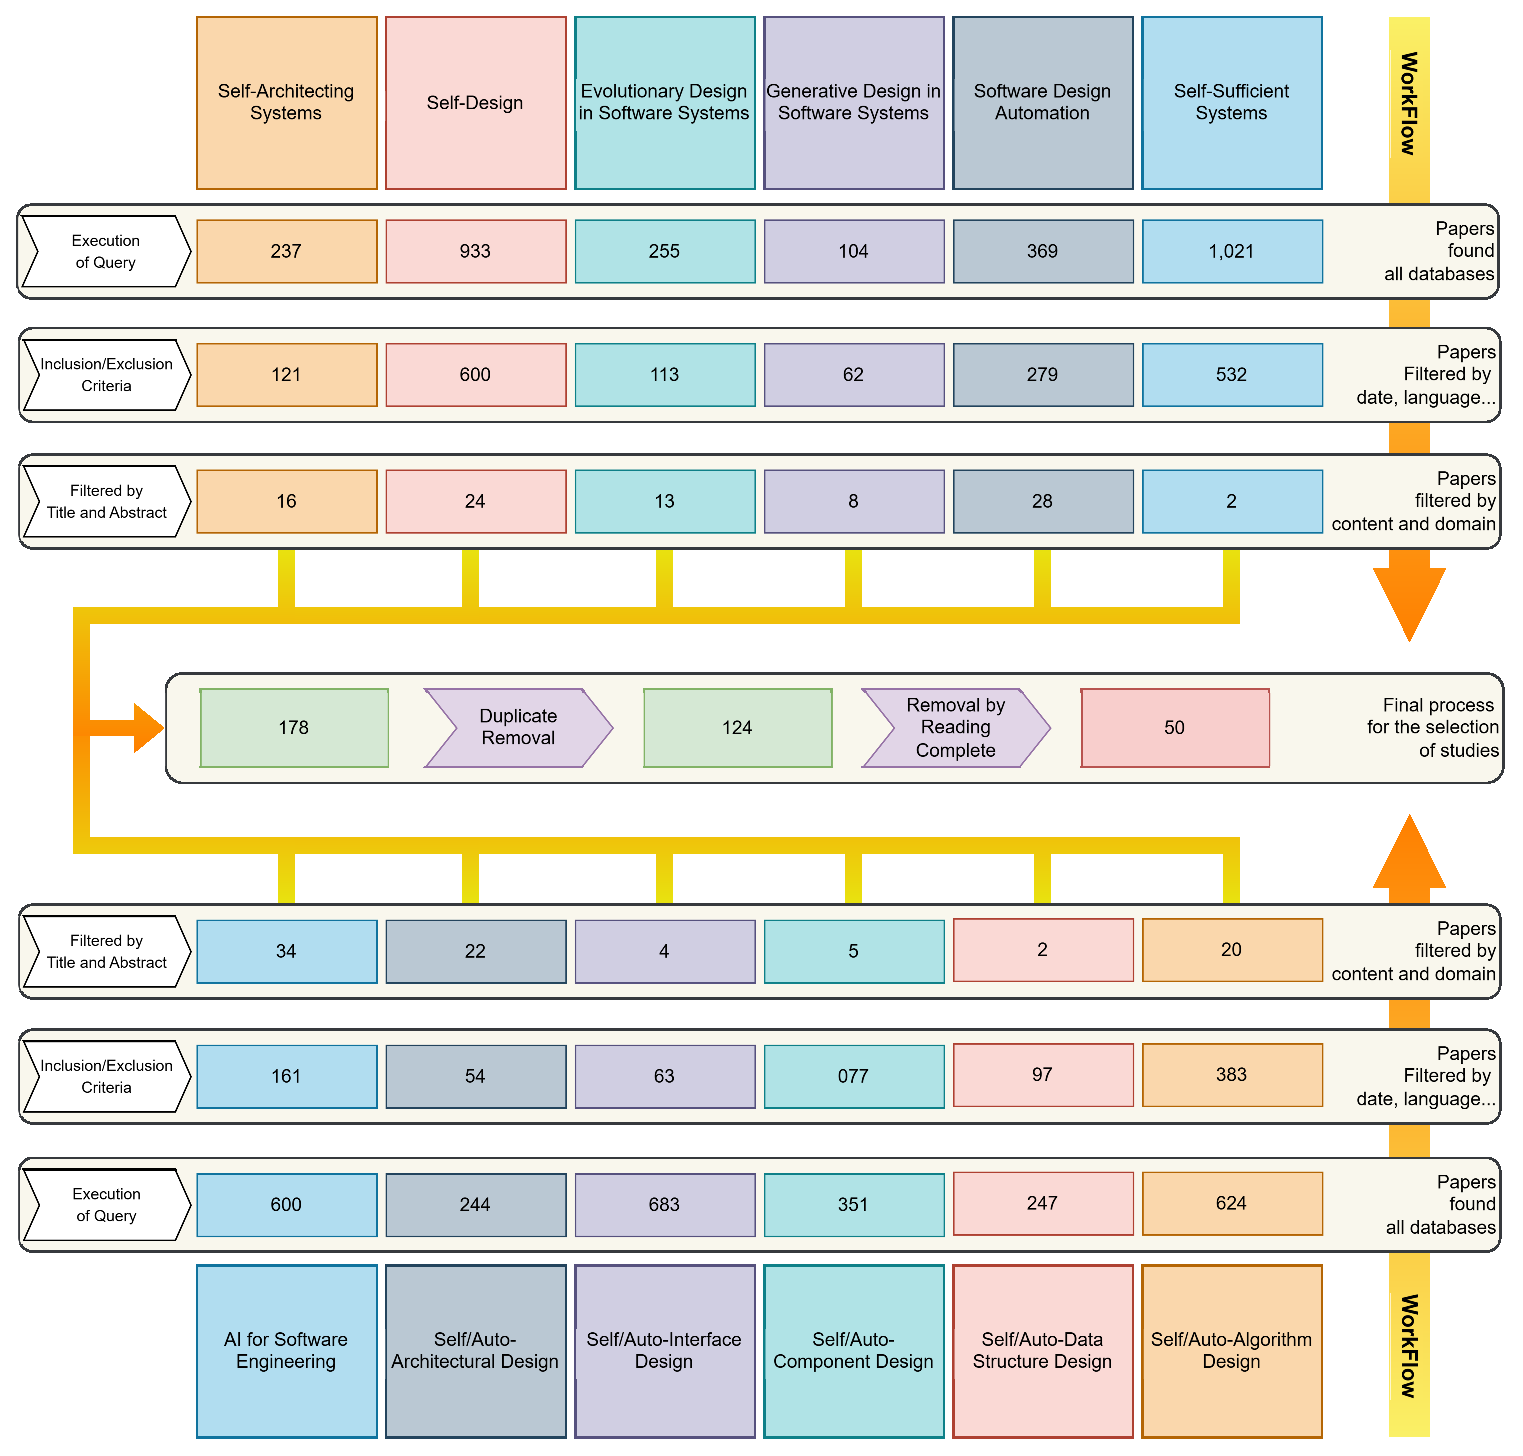
\includegraphics[width=0.9\textwidth]{figures/Fig2_StudySelection.eps}
	\caption{Proceso de seleccion de articulos con resultados cuantitativos por etapa de cribado.}
	\label{fig:Cribado}
\end{figure}

\subsubsection{Extracción de datos}

La extracción de datos se realizó exclusivamente a partir de los estudios que cumplían con los criterios de inclusión definidos y presentados en la Tabla~\ref{tab:criterios}. Este proceso se llevó a cabo de manera sistemática para garantizar la coherencia y la trazabilidad de la información recopilada de cada estudio seleccionado. Dada la heterogeneidad de la literatura analizada, se empleó un análisis narrativo para sintetizar la información. En este contexto, los enfoques analizados se organizaron en categorías temáticas derivadas de los objetivos de la revisión y de las preguntas de investigación formuladas. Esta estrategia permitió identificar patrones recurrentes, tendencias emergentes y áreas poco exploradas dentro de los estudios seleccionados. Asimismo, la estructuración temática facilitó una evaluación comparativa de cómo cada estudio aborda el autodiseño en el contexto de la ingeniería de software, destacando las similitudes y diferencias entre los enfoques propuestos, así como el grado en que sus hallazgos contribuyen a responder a las preguntas de investigación planteadas en esta revisión.

\subsubsection{Resultados}

Los resultados completos están en la publicacion titulada "Automated Software Design Towards Zero Human Intervention: A Systematic Literature Review", pero para este trabajo estan implementados en el Marco Teorico y mayormente en Estado del Arte.

\subsubsection{Discusión}
La siguiente es una síntesis de lo que fue la discusión completa.

La revisión revela un punto de inflexión hacia la automatización del diseño de software a través de cuatro paradigmas principales: la refactorización basada en búsqueda (SBR), el autodiseño algorítmico mediante mejora genética (GI), la adaptabilidad formal con ontologías y planificación (PDDL), y la transición hacia la Ingeniería de Software 3.0 (SE 3.0) basada en ecosistemas multiagente. Aunque estos enfoques permiten manipular arquitecturas complejas y redefinen el rol del desarrollador hacia el de un orquestador estratégico, enfrentan importantes desafíos técnicos: la pérdida de semántica en los modelos matemáticos, la inestabilidad durante el reemplazo de código en caliente, la sobrecarga computacional en entornos inciertos y el riesgo de alucinaciones de diseño ante la falta de restricciones verificables y gobernanza en los agentes. Finalmente, se evidencia una brecha crítica entre el potencial teórico y la práctica, ya que la mayoría de los estudios se limitan a entornos controlados o sintéticos; por ello, se concluye que la integración del razonamiento simbólico con modelos de lenguaje es indispensable para lograr arquitecturas autogeneradas transparentes, funcionales y viables en entornos de producción reales.

\subsection{Definicion y conceptualizacion}



\subsection{Uso de Prometheus}



\subsection{Analisis y validacion}



\section{Propuesta marco conceptual y arquitectura}



\subsection{Definicion conceptual y formal}



\subsection{Propuesta detallada}



\subsection{Resumen Conceptual}



\chapter{Experimentación y Análisis de Resultados}



\section{Análisis de selección automática de algoritmos}



\subsection{Análisis de la arquitectura: auto-diseño}



\section{Experimentación}



\subsection{Caso de estudio: nuevo problema, nueva solución}



\subsection{Experimento: Identificación del Problema}



\subsection{Experimento: Identificación del Algoritmo}



\chapter{Conclusiones y Trabajo Futuro}



\section{Conclusiones}



\section{Objetivos logrados}


\section{Trabajo a futuro}





% ---------------------------------------------------------
% REFERENCIAS Y APÉNDICES
% ---------------------------------------------------------
\printbibliography[title={Referencias Bibliográficas}, heading=bibintoc]

\appendix
\chapter{Código Fuente Relevante}


\end{document}